\section{Results}
\label{sec:results}

\begin{figure}
  \centering
  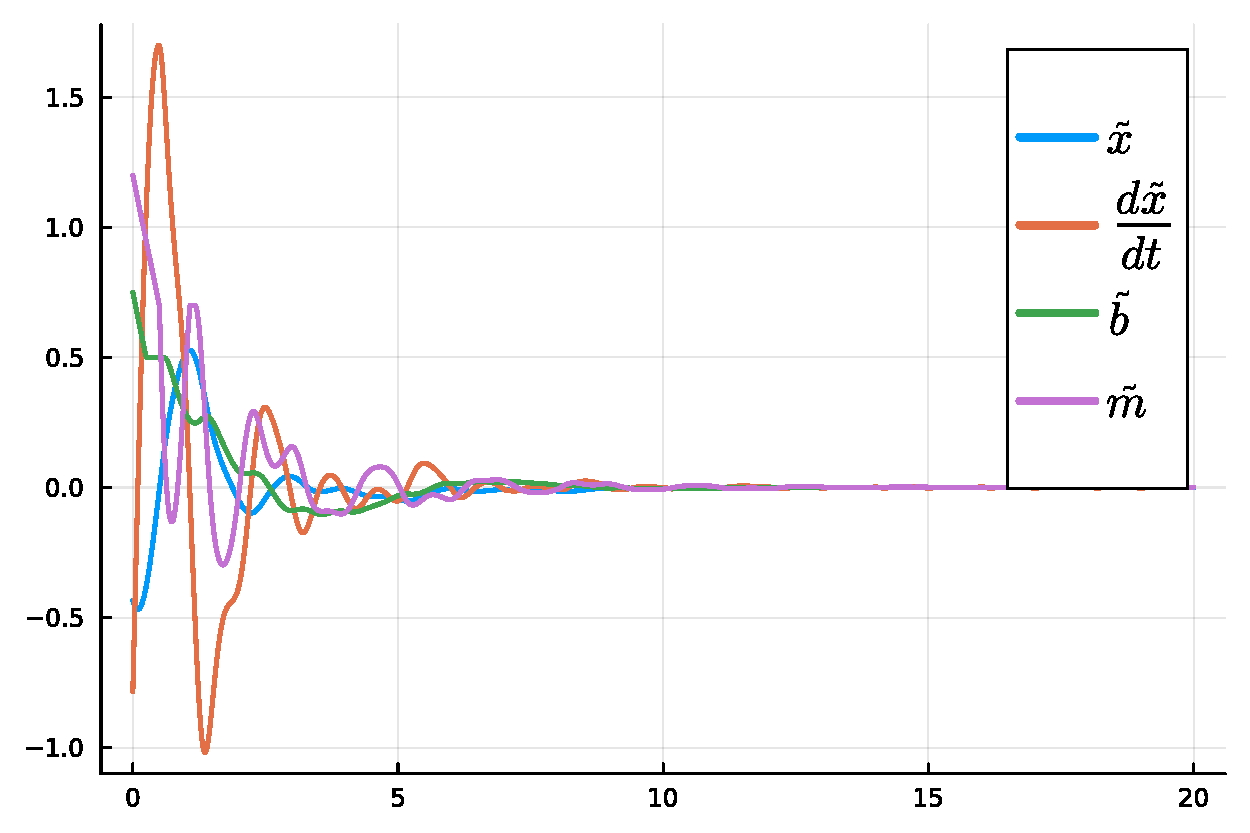
\includegraphics[width=0.5\textwidth]{./figures/adaptationrule2.pdf}
  \caption{Simulation showing that the system and estimation errors converge to
  zero.}
  \label{fig:adaptation}
\end{figure}

In Figure~\ref{fig:adaptation}, we plot the response of the system to the
control and adaptation laws laid out in Section~\ref{sec:analysis} with $(A,
\omega, \varphi) = (\nicefrac{1}{2}, \pi, 60^\circ)$ and $(k, \lambda) = (1,
1)$. The real mass and damping of the system is $(m, b) = (0.7, 0.5)$ and their
estimates start at $(\hat{m}, \hat{b}) = (-\nicefrac{1}{2}, -\nicefrac{1}{4})$.
